
\label{ch:Context théoritique}

\section{Introduction}

Dans cette section, on va décrire quelques notions mathématiques de la théorie derrière le vocodeur de phase. Pour embrasser la théorie de la dissolution spectrale, il faut accepter qu'un signal complexe, signifiant autre chose qu'une simple onde sinusoïdale, puisse être représenté par une série de chevauchements de simples sinusoïdes d'amplitudes et de fréquences différentes.

Pour visualiser cette méthode, le paradigme de la synthèse additive peut être utilisé comme une construction inverse. Une méthode classique de synthèse d'un son complexe variant dans le temps consiste à combiner plusieurs formes d'ondes élémentaires. Les formes d'ondes qui se superposent à la synthèse additive sont souvent sinusoïdales. Dans certaines conditions, les sinusoïdes individuels fusionnent et le résultat est perçu comme un son riche et unique.

L'idée derrière cette méthode n'est pas nouvelle. En effet, la synthèse additive est utilisée depuis des siècles dans des instruments traditionnels tels que l’orgue.

Lorsqu'un son presque périodique est analysé, son énergie spectrale est concentrée autour de quelques fréquences discrètes (harmoniques). Ces fréquences correspondent à différents signaux sunisoïdaux appelés partiels. L'amplitude de chaque partiel n'est pas constante et sa variation dans le temps est cruciale pour la caractérisation du timbre, spécialement dans la phase transitoire initiale d’une note (attaque). On peut toutefois penser que la fréquence de chaque composante varie lentement. La synthèse additive consiste de la somme d'oscillateurs sinusoïdaux dont l'amplitude et la fréquence varient dans le temps. Les paramètres de contrôle sont déterminés par une analyse spectrale.

\section{Décodage mathématique}

    \subsection{The Fourier Transform}

L’analyse spectrale consiste essentiellement à passer du domaine temporel au domaine fréquentiel pendant une période temporelle fixée. De ce point de vue, l’analyse spectrale est une transformation de Fourier associée à un processus mathématique permettant de visualiser les fréquences qui composent une onde sonore complexe pendant une période temporelle fixée.

Il existe de nombreuses façons de calculer la transformation de Fourier discrète (DFT), dont la FFT. Bien que toutes les méthodes DFT soient converties en un même résultat, la FFT est l’une des méthodes de calcul les plus efficaces. La FFT est l’un des algorithmes les plus utilisés en traitement du signal en raison de la quantité minimale de code nécessaire à sa programmation. Néanmoins, il fait partie des algorithmes les plus difficiles du domaine DSP.

La FFT est un algorithme complexe, dans le sens où il utilise des nombres complexes pour s'exécuter. En raison de sa complexité, les détails techniques sont fréquemment omis et laissé pour un contexte peut-être pure mathématique.

Le processus de DFT est expliqué graphiquement dans la figure \ref{ComplexDFT}. Dans la colonne de gauche, on peut voir la représentation temporelle du signal. En conséquence, dans la colonne de droite, la transformation FFT peut être visualisée dans le domaine fréquentiel. $ N $ est la taille de la fenêtre en termes de DSP ou la durée totale de l'analyse en général. Comme le montre la figure \ref{ComplexDFT}, le signal est décomposé en variables à 2 axes, un réel et un imaginaire.

\begin{figure}
    \centering
    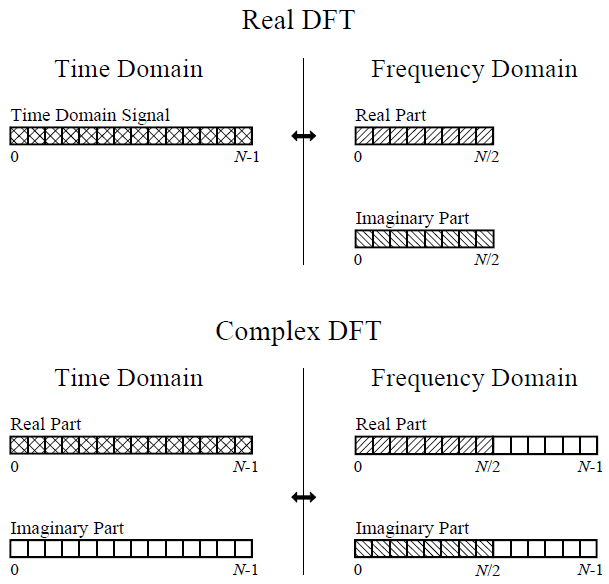
\includegraphics[width = 0.5 \textwidth ]{Graphs/ComplexDFT.png}
    \caption{Complex DFT}
    \label{ComplexDFT}
\end{figure}

En 1822, Jean Joseph Fourier montra que certaines fonctions semi-périodiques peuvent également être formulées comme une somme d'harmoniques:
 
\begin{equation}\footnote{Curtis Roads. The Computer Music Tutorial. MIT Press, Cambridge, MA, USA, 1996. ISBN 0262680823.[p. 1085]}
    x(t) = c_0 + \sum_{n=1} ^ \infty c_n cos( \omega t + \theta_n) 
\end{equation}

Où $ t $ est la période, $ x $ est le signal, $ c_0 $ est l'harmonique fondamentale, $ f $ la fréquence, $ \omega = 2 \pi f $ et $ \theta $ est la phase de chaque harmonique . Dans cette formulation de la transformation de Fourier, il est clair qu’un son $ x $ lié au facteur de temps $ t $ peut être décrit comme une somme de sinusoïdes.

Pour cette raison, la transformation de Fourier pour toute fonction intégrable $ f: \mathbb{R} \to \mathbb{C} $ est la suivante :
 
\begin{equation}\footnote{Hermann L F. Helmholtz. The Sensations of Tone. New York, 1895.[p. 215]}
     F[x(t)](\omega) = \int_{-\infty}^{+\infty} e ^ {-j \omega t} x(t) \hspace{1mm} dt \hspace{5mm} 
\end{equation}
    
Où $ F[x(t)] (\omega) $ est la transformation de Fourier du signal $ x $ bornée par sa  fréquence $ \omega $ correspondante. Dans le domaine sonore numérique, cette fréquence varie entre 0 et la fréquence d'échantillonnage (SR). Le SR est généralement de 44100 ou 48000Hz. Le domaine de cette fonction pouvant être intégrée aux signaux sonores numériques varie dans l'intégrale $ [- 1, 1] $. Comme on le voit clairement dans cette formule, le foncteur temporel est infini, mais un tel calcul est évidemment impossible. D'autres variations de la transformation de Fourier en temps discret sont en réalité utilisées en informatique.

         \begin{figure}
            \centering
            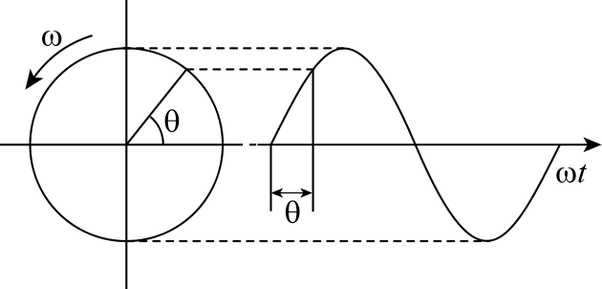
\includegraphics[width = 0.5 \textwidth ]{Graphs/Fourier_Circle_1.png}
            \caption{Circle de la transformation Fourier}
            \label{CircleFourier}
        \end{figure}

La transformation de Fourier est basée principalement sur la formule d'Euler où $ e ^ {2 j \pi t} = cos (2 \pi t) + j sin (2 \pi t) $. On peut imaginer cette opération comme dessiner un cercle dans le plan complexe $ \mathbb{C} $. Au cours de la transformation de Fourier, un signal $ x(t) $ est rendu autour d'un cercle avec ($ e ^ {- j \omega t} $), avec une fréquence $ f $. Rappelons que $ \omega = 2 \pi f $. La rotation est donnée par le signe de $ j $ (nombre imaginaire). Une rotation dans le sens des aiguilles d'une montre est donc considérée comme $ -j $. Ce processus nous donne effectivement deux parties, la vraie, $ cos (2 \pi) $, et l’imaginaire, $ j \; sin (2 \pi t) $,  partie de l'équation.

On transformerait souvent les données cartésiennes induites par l'exponentielle complexe en une forme polaire plus familière. Après la transformation de Fourier, il existe deux facteurs à manipuler, la phase et la magnitude. La phase est induite par l'angle des deux coordonnées cartésiennes dans le plan complexe tandis que la magnitude est déduite par le vecteur produit des deux valeurs. De la phase, on peut extraire des informations sur la fréquence du signal sur l'échantillon précise et, comme son nom l’indique, des informations de magnitude sur l’amplitude de l’échantillon exacte. Lorsque le temps est fixé pour l'exécution de l'analyse de Fourier, le signal sonore est divisé en intervalles de fréquence factorisés par la fréquence de l'analyse ($ \omega $). La phase et la magnitude sont calculées pour chaque fraction de temps sur laquelle l'analyse de Fourier est effectuée. La magnitude est égale à: $ m (x) = \sqrt{i (x) ^ 2 + r (x) ^ 2} $ et la phase est $ \theta (x) = tan ^ {- 1} (\frac{i (x)}{r (x)}) $. \ref{MagnitudePhase}

         \begin{figure}
            \centering
            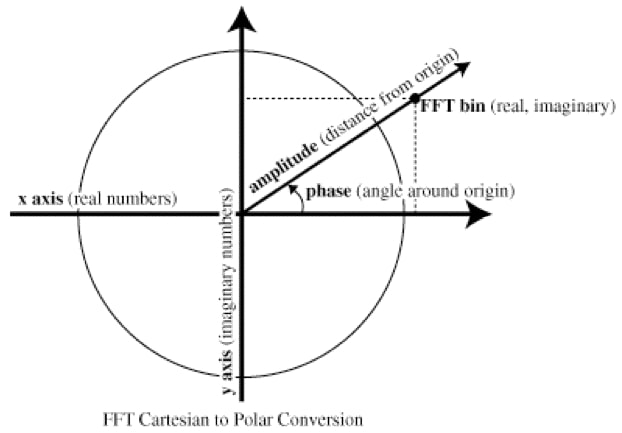
\includegraphics[width = 0.5 \textwidth ]{Graphs/Fourier_Circle_2.jpg}
            \caption{Magnitude et phase}
            \label{MagnitudePhase}
        \end{figure}

Évidemment, dans le domaine numérique, on ne peut pas utiliser une partie de temps infinie. Nous introduisons, donc, la notion de la fenêtre et, ainsi,  de fenêtrage. La fenêtre est une période de temps exprimée en images. Les images sont une notion équivalente du SR en ce sens que le SR calcule une quantité d'images du son par minute et que les images sont exactement ces images. Une analyse fenêtrée est généralement exprimée par un algorithme de transformation à court terme de Fourier (STFT) \footnote{Jown Strawn, \textit{STFT : Short Time Fourier Transform}, 1985, pp. 141– 134.}.

\begin{equation}
\footnote{Tadej Droljc. STFT Analysis Driven Sonographic Sound Processing in Real-Time using Max/MSP and Jitter. 2011.}
    X(\omega, \tau) = \sum_t ^ \infty x(t) \omega(t-\tau)e ^ {-j \omega t} \hspace{5mm} 
\end{equation}

Où $x$ est le signal, $X$ sa transformation Fourier (une abréviation de la forme $F[x(t)]$), $\omega = 2 \pi f$ , $t$ le temps continue, $\tau$ l’instant temporel, $c_n$ les harmoniques, $\omega(t)$ le fenêtrage, et $j$ un nombre complexe.

Dans cette recherche, on va utiliser la forme continue TFD et puis FFT, vu que cette formule est premièrement utilisée dans MaxMSP et en plus requiert une puissance calculatrice plus efficiente que d’autres méthodes :

\begin{equation}
\footnote{Jean-François Charles. A tutorial on spectral sound processing using maxmsp and jitter. Computer Music Journal, pages 87–102, Printemps 2008.}
    X(\omega) = \frac{1}{N} \sum_{n = 0} ^ {N-1} x(n+1) e ^ {-j \frac{\omega n}{N}} \hspace{5mm}
\end{equation}

Où $ N $ est la taille de la fenêtre, qui correspond au nombre total d'images qu'il contient. $ X $ est le signal, $ n $ énumère chaque image dans $ N $ et $ \omega = 2 \pi f $ comme d'habitude mais dans cette version, f varie entre 0 et N. Nous le présenterons plutôt comme $ \omega = 2 \pi k $ où k représentera la $ k-$ième harmonique.

Pour chaque transition vers le domaine fréquentiel, une fonction inverse du domaine temporel est nécessaire. La fonction inverse se caractérise par la transformation de Fourier rapide inverse (IFFT) pour des valeurs de temps discrets.

\begin{equation}
\footnote{Alan V. Oppenheim et Ronald W. Schafer. Discrete-time signal processingd. Prentice Hall Press.}
    x(n) = \frac{1}{N} \sum_{ f = 0} ^ {N-1} X(f) e ^ {j \frac{2 \pi f n}{N}} \hspace{5mm} 
\end{equation}

    \subsubsection{Transformation Fourier rapide (FFT)}

C'est toujours bien d'avoir un point de base théorique, mais ce qui compte vraiment, ce sont les formules computationnelles. Par computation, nous entendons une formule qui est facile à exécuter par un ordinateur en temps raisonnable et à produire une sortie. Une solution à cette affirmation est la transformation de Fourier rapide. Ainsi, FFT est un algorithme calculable pour DFT qui utilise un moyen intelligent pour réduire le temps de calcul et la complexité des calculs.

Nous rappelons la DFT standard interprétée dans du code informatique.

\noindent\begin{minipage}{\textwidth}
    \begin{lstlisting}[language=Python, caption= DFT]
    function DFT(x)
        N = length(x)
        # We want two vectors here for real space (n) and frequency space (k)
        n = 0:N-1
        k = n'
        transform_matrix = exp.(-2im*pi*n*k/N)
        return transform_matrix*x
    end.
    \end{lstlisting}
\end{minipage}

Il est clair que la transformation de Fourier est en réalité une matrice de calcul. Cependant, en effectuant autant de calculs, on peut imaginer que le processus est assez cher computationnellement. Les conditions requises pour la DFT sont le traitement en temps réel et des fenêtres d’une taille minimale de 512 échantillons pour les données sonores. L'amélioration de l'algorithme a été donnée par James Cooley et John Tukey \footnote{James Cooley et John Tukey, \textit{Un algorithme pour le calcul automatique de séries de Fourier complexes}, 1965. \nocite{Fourier_complex}}
 
L'algorithme de Cooley-Tukey utilise la récursivité pour réduire la complexité de calcul. En particulier, la matrice produite par la réduction dans le domaine fréquentiel est réduite en deux parties avant d'effectuer les calculs DFT. Nous séparons les indices impairs des casiers du même, puis la procédure est répétée. Ce processus réduit la complexité à $ \mathcal{O} (n \; log \; n) $ à partir d’une taille polynomiale. Bien sûr, pour effectuer cette action en raison de la division continue par deux, nous demandons que la fenêtre d’analyse soit une puissance de deux.

Le diagrammes au forme de “Butterfly” est l'idée principale de la réduction du calcul FFT. En particulier, Cooley et Tukey ont remarqué que les exponentielles complexes sont entièrement répétées dans la seconde moitié de la fenêtre avec un signe opposé. Par conséquent, en divisant constamment la vidéo, les calculs de l’exponentielle complexe sont considérablement réduits. Nous pouvons visualiser le processus dans la figure \ref{Butterfly} \footnote{Image récupérée de l'article: \href{https://www.researchgate.net/figure/Radix-2-butterfly-diagram-for-8- point-FFT_fig1_312460770}{P. G. Reshma, P. Gopi Varun, Babu V. Suresh, Wahid Khabou, \textit {Analog implementation of FFT using cascade current mirror}, 2017.}}.

    \begin{figure}
        \centering
        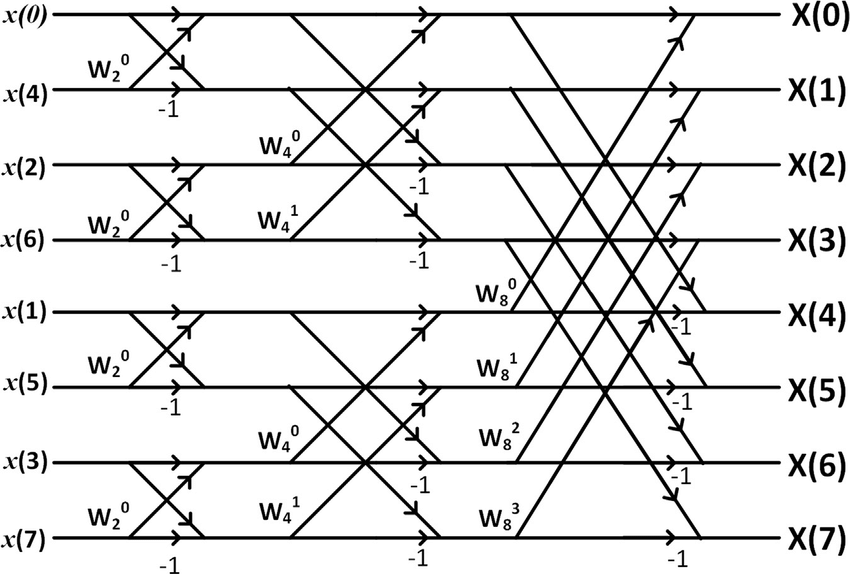
\includegraphics[width = 8cm]{Graphs/Butterfly_8-point-FFT.png}
        \caption{Butterfly Diagrams for an 8 point FFT}
        \label{Butterfly}
    \end{figure}

Une mise en oeuvre du code correspondant est en disposition dans l'appendix \ref{Cooley-Tukey_Code}.

\subsection{Fenetrage}

Pour calculer le STFT, il faut définir la taille de la fenêtre à traiter. La transformation de Fourier dans une fenêtre temporelle discrète peut produire des artefacts contredisant le continuum du signal. Pour éviter cet effet, il est habituel de multiplier la fenêtre du son d'origine par une fenêtre, qui ne contient pas des informations sonores, de la même taille sur laquelle une fonction factorise l'amplitude du son. La transformation de Fourier est reproduite un nombre dénombrable de fois en fonction de la taille du son analysé. La fenêtre est généralement beaucoup plus petite que le son d'origine, ce qui la répète plusieurs fois pendant toute la durée du son. Il est important que la fenêtre soit déplacée dans le temps, mais elle est également se chevaucher par un facteur. Le processus peut être décrit visuellement dans la figure \ref{overlapping}.

Cette technique, appelée chevauchement où superposition, donne un résultat sonore plus arrondi. En raison du chevauchement et de la multiplication envellop, l'auditeur ne peut percevoir aucun des artefacts possibles induits par l'analyse mais on entend un résultat unifié \footnote {Daniel W. Griffin et Jae S. Lim. Estimation du signal à partir de la transformation de Fourier à court terme modifiée. IEE Transaction sur l'acoustique, la parole et le traitement du signal, ISSE Vol. 32: 236-243, avril 1984.}. 
 
         \begin{figure}
            \centering
            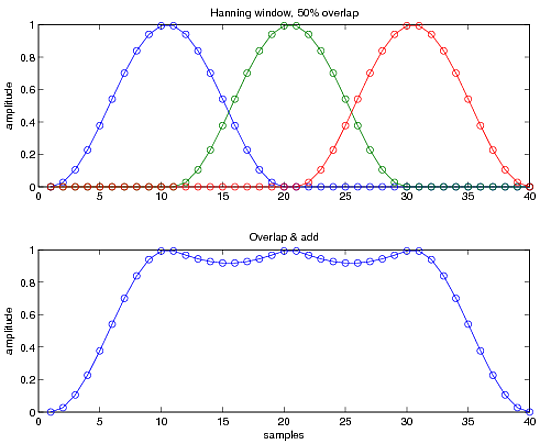
\includegraphics[width = 0.5 \textwidth ]{Graphs/Overlapping.png}
            \caption{Overlapping}
            \label{overlapping}
        \end{figure}

\subsubsection{Filtres Gabor}

Ici, nous examinerons la possibilité d’utiliser des filtres de Gabor pour appliquer un envelop au signale sonore. Les filtres de Gabor sont définis comme la multiplication continue d'une fonction gaussienne par un signal complexe bornée par un facteur temporel. Le filtre gaussien est décrit dans la formule suivante:

\begin{equation}
    G_x(t,f) = \int_{-\infty}^{+\infty} e ^ {-\pi(\tau-t)^2} e ^ {-j\omega \tau} x(\tau)\hspace{1mm} d\tau  
\end{equation}

Il est possible de considérer un filtre de gabor comme deux filtres déphasés se produisant en décomposant le complexe exponentiel par rapport à une partie imaginaire et réelle. Où la partie réelle a le filtre $ g_ {real} (t) = w (t) péché (2 \pi f_k t + \theta) $ et la partie imaginaire $ g_{ima} (t) = w (t) cos (2 \pi f_0 t + \theta) $.

Les deux filtres peuvent être déphasés mais la phase de prise en compte. Par conséquent, leur effet sur une sinusoïde est toujours une sinusoïde.

Pour manipuler la courbe d'un filtre de Gabor, il suffit de changer les paramètres. La formule normalisée se transforme en:

\begin{equation}
    G_x(t,f) = \int_{-\infty}^{+\infty} \frac{1}{\sigma \sqrt{2 \pi}} e ^ {-\frac{1}{2}(\frac{\tau-t}{\sigma})^2} e ^ {-j\omega \tau} x(\tau)\hspace{1mm} d\tau  
\end{equation}

Where $\sigma$ is the parameter of the Gaussian curve. A Gabor filter will allow to create a smoother sound result after Où $ \sigma $ est le paramètre de la courbe gaussienne. Un filtre de Gabor permettra de créer un résultat sonore plus lisse après l'analyse.

La même logique est valable pour tous les types d’un evelop de fenêtre tels que le hanning, le hamming, etc.

    \subsection{Le vocodeur de phase}    
    
        \subsubsection{Définition}   

Le vocodeur de phase est un outil d'analyse-synthèse qui utilise la DFT. L'analyse est effectuée de sorte que le signal de sortie ne subisse aucune perte de données de la transformation, que ce soit théoriquement ou concrètement. Le signal de sortie est identique à l'entrée avant l'analyse si aucun traitement n'est appliqué. Les utilisations les plus courantes du vocodeur de phase sont le décalage de hauteur de ton et l’alternance de la vitesse de lecture. Le vocodeur de phase n’a pas de restriction évidente et peut également garder une trace des inharmonicités et du vibrato des sons \footnote {Johannes Grünwald. \textit{Theory, implementation and evaluation of the digital phase vocoder in the context of audio effects}, 2010.}.

        \subsubsection{Histoire} 

Le vocodeur de phase a été introduit, en 1966, par Flanagan en tant qu'un algorithme préservant la cohérence horizontale entre les phases des segments représentant les composants sinusoïdaux. Le vocodeur de phase n'a pas pris en compte la cohérence verticale produite par les intervalles de fréquences adjacentes et, par conséquent, l'étirement temporel du système a produit des signaux sonores avec une perte de qualité. La reconstruction optimale du signal de la STFT après traitement a été proposée par Griffin et Lim \footnote{Daniel W. Griffin et Jae S. Lim, \textit{Signal estimation from modified short-time fourier transform}, 198, pp. 236–243.} en 1984. Cet algorithme ne considérait pas produire un STFT cohérent, mais plutôt rechercher le signal optimal dont le STFT est aussi proche que possible du STFT modifié, même si le STFT modifié n'est pas cohérent (ne représente aucun signal).

Le problème de la cohérence verticale était un problème majeur pour la qualité opérationnelle à l'échelle temporelle jusqu'en 1999. A cette époque, Laroche et Dolson \footnote{Mark Dolson, \textit{The phase vocoder : a tutorial}, 1986, pp. 14-27.} ont proposé un moyen de préserver la cohérence phase des composantes spectrales. Le développement de Laroche et de Dolson doit marquer un tournant dans l’histoire du vocodeur de phase. Il a été prouvé que, grâce à la cohérence de phase, une transformation temporelle de haute qualité peut être obtenue.

Néanmoins, l'algorithme découvert par Laroche et Dolson n'a pas pu conserver la phase verticale à l’attaque d’un son. Roebel a proposé une solution à ce problème \footnote{Axel Roebel, \textit{ Morphing sound attractors}, 1999.} en 1999. Un exemple mis en oeuvre du vocodeur de phase utilisant la dernière version de Roebel est constitué par les outils SuperVP de l’Ircam.

Une approche à la description du vocodeur de phase consiste à représenter le signal une séquence des images successives d’une transformation de Fourier Discrète (TFD) d’une fenêtre de longueur $ N$. Ces images sont d'abord multipliées par une fenêtrage appropriée (telle que Hamming, Hanning, Kaiser, Blackman, etc.) puis transformés dans le domaine fréquentiel. A ce stade, toute modification prudente du spectre peut être faite, avant la transformation inverse au domaine temporel avec la transformation de Fourier discrète inverse (TDFI). Là, les parties d'overlap et éventuellement fenêtrées sont additionnées, ce qui donne le résultat final.

\vspace{0.4cm}

La STFT (une transformation caractérisée des successions des TFD) d'un signal fenêtré est défini comme suit:

\begin{equation}
    x(n) = \frac{1}{N}\sum_{ k = 0 }^{ N-1 } X_f (n)W_N \hspace{0.05cm}^{ nf}, \hspace{1cm} \forall n \in SR 
\end{equation}

ou \hspace{0.1cm} $ W_N = e ^ {\frac{2\pi j}{N}} $ \hspace{0.1cm} et $ h(n) $ est une fenêtre approximativement choisie.

\begin{equation}
    h_f(n) = \frac{1}{N} h(n) W_N \hspace{0.05cm} ^{nf},\hspace{1cm}  k = 0, 1, \dots, N - 1 
\end{equation}

Pendant le processus de l'analyse, la succession des images d'une STFT font parties du signal d'entrée $x(n)$, sur la position $n_a^u = uR_a$, ou $R_a$ est nommé \textit{input hop size} et $u$ doit etre un entier. La fenêtre(ou la durée) de la DFT est définie par la taille $N$, ou le \textit{hop size} est forcément une sous-multiplication de $N$. Cet effet permettra de réaliser un \textit{overlap} de 50\%, 75\%, etc.

Le terme $\tilde{x}_u(n)$ propose l'estimation des fenêtres symétriques calculées. Donc si nous supposons un chevauchement du fenêtrage par 50 \%, ou bien $N/2$, on propose une manière d'éviter les asymétries de phase ci-dessus:  

\begin{equation}
    X[n_a^u, \omega] = \sum_{n=0} ^{N-1} \tilde{x}_u(n) e^{-j \omega \frac{n}{N}} \vspace{0.5cm} 
\end{equation}

\hspace{5cm} ou \hspace{1cm} ${x}_u(n) = h_a(n) x(n-n_a^u)$ 

Le terme $\tilde{x}_u(n)$ propose l'estimation des fenêtres symmetriques calculées. Donc si nous supposons un overlap de fenetrage par 50 \%, ou bien $N/2$, puis une maniere d'eviter les assymetrages de phase est composée ci-dessus:  

\begin{equation}
    \tilde{x}(n) = x[((n-N/2))_N] 
\end{equation}

ou $((.))_N$ présente l'opération du modulo, et $N$ est la durée de la fenêtre et il devait être un pair.


Donc la transformation de Fourier du signal liée au fenêtrage devient :

\begin{equation}
    X(rl,f) = \sum_{N=0}^{N-1} x(n) h(rl-n) e^{-j \frac{2 \pi}{N} fn}
\end{equation}

C'est une fonction de deux variables discrètes, le temps $ rl $ et la fréquence $ k $. L'indice $ ir $ est la position de la fenêtre, $r$ étant le numéro de l’échantillon et $l$ la taille du pas de chevauchement de la fenêtre d'analyse. $ S (rl, k) $ peut être vu comme le spectre de la multiplication $ s (m) w (rl-m) $, qui est la séquence en entrée s (m) multipliée par la fenêtre décalée à la position $ rl $. Ce n'est pas le spectre exact, mais sa convolution avec la transformation de Fourier des fenêtres correspondantes.

C’est, donc, une fonction de deux variables discrètes, le temps rl et la fréquence f. L’index rl
est la position de la fenêtre, r étant le numéro d’image (frame) et l la taille du décalage de la
fenêtre d’analyse.

$ X (rl, f) $ peut être vu comme le spectre de la multiplication $ x (n) h (rl-n) $, qui est le signal d'entrée $ x (n) $ multiplié par la fenêtre décalée à la position $ rl $. Ce n'est pas le spectre exact, mais sa convolution avec la transformation de Fourier de la fenêtre.

La procédure standard de chevauchement (\textit{overlap}) consiste à additionner les buffers et à les diviser par la somme des fenêtres décalés. Le signal de sortie y(n) est exprimé comme:

\begin{equation}
    y(n) = \frac{\sum_r \bar{x}(rl,n)}{\sum_r {h}(rl - n)})
\end{equation}

Pour construire une reproduction du signal d'origine ou du signal transmuté après traitement, un iFFT est nécessaire. Dans le vocodeur de phase, cette procédure accède aux informations de phase et d'amplitude et se forme comme suit:

\begin{equation}
    \bar{s}(rl,k) = \frac{1}{N}\sum_{k=0}^{N-1} |\bar{S}(rl,k| e^{j (\frac{2 \pi}{N} km + \theta(r \bar{l},k))}
\end{equation}

Enfin pour calculer la fréquence de chaque image instantanée il suffit de suivre la formule :

\begin{equation}
    \bar{f}_{k,r} = \frac{\theta(rl,k) - \theta((r - l )l,k)}{l}
\end{equation}

\subsection{Applications du vocodeur de phase} 

    \subsubsection{Time Streching}

Pour réaliser un étirement du temps d'un son, traditionnellement, il suffit de baisser ou augmenter le rythme de sa lecture, mais cela produit également un changement de la hauteur. Le vocodeur de phase permet d'effectuer un étirement temporel sans pour autant changer la hauteur ou la qualité sonore. Afin de mieux comprendre le fonctionnement du vocodeur il faut considérer la transformation Fourier à court terme, pour un étirement temporel. Pour visualiser le résultat on peut imaginer, que pour chaque période de temps de la transformation Fourier appliquée, une série des harmoniques sauvegardées dans une fenêtre, et le facteur de son overlap. Il suffit d'éloigner ou rapprocher les fenêtres, pour changer le rythme de la lecture sans affecter la hauteur sonore.

Le modèle qui correspond à l'étirement temporelle est donnée par la formule suivante :

    \begin{align}
         x(n) &= \sum_{k=1}^{K(n)} A_k(n) \; e^{j \theta_k (n)} \\
         \theta_k(n) &= \theta_k(0) + \int_{0}^{n} f_k (\tau) \; d\tau
    \end{align}

Ou un signal est interprété par une somme des sinusoïdes $K(n)$ avec leur magnitude $A_k(n)$ et phase $\theta_k$ appropriées. Par la suite, la phase instantanée du $k-$ième sinusoide, $\theta_k(n)$, est calculée par l'addition de la phase de la première échantillon $\theta_k(0)$ avec l'intégrale des fréquences $f_k (n)$. Le dernière est équivalent à $\Sigma_{n=0}^N f_k(n)$ pour une transformation discrète.

La modification temporelle est déterminée par deux paramètres parallèles, c’est à dire la modification de phase instantanée pour chaque échantillon et la modification du fenêtre du décalage (hop window). Plus précisément, le \textit{hop window} du stade de l'analyse est différent du \textit{hop window} de la synthèse.

Pour une modification temporelle par un facteur constant $\alpha$ tel que $n_k^u = \alpha n_\alpha^u$ la phase d'un étirement temporel devient \footnote{Jean Laroche et Mark Dolson, \textit{Improved Phase Vocoder}, 1999, p. 324 \nocite{DoLa99}}:
    
    \begin{equation}
        \theta_k^(n_k^u) = \theta_k(0) + \alpha \int_0^{n_k^u}  f_k (\tau) \; d\tau
    \end{equation}

    \subsubsection{Transposition de l'hauteur}

Comme le vocodeur de phase peut être utilisé pour réaliser un étirement temporel d'un son sans affecter sa hauteur, il devrait également être possible de faire l'inverse, c’est-à-dire changer la hauteur sans changer le rythme de la lecture. En effet, cette opération est facilement accomplie. La procédure est de changer le rythme de la lecture par le facteur de changement de la hauteur souhaitée, puis de jouer le résultat sonore produit à la fréquence d'échantillonnage \guillemotleft incorrecte \guillemotright. Par exemple, pour augmenter la hauteur d’une octave, le son est d'abord agrandi d'un facteur de deux, et il est ensuite joué à deux fois l'original taux d'échantillonnage. \footnote{Mark Dolson, \textit{ The phase vocoder}, 1986.}

    \subsubsection{Freeze}

À cet effet, nous prenons un certain fenêtre d’analyse à partir du son sélectionné et nous «gèlons» ce son dans le temps. Pour achever cet effet il s'agit de rendre le rythme de la lecture de notre vocodeur de phase au zéro. Cela peut se comparer à un étirement sonore infini. On peut ainsi appliquer les mêmes principes d'un étirement sonore normal.

    \subsubsection{Robotisation}

Pour faire une robotisation d'un signal il faut mettre la phase de chaque echantillon à zero. Cet effet resulte à un son robotisé et métalique.

    \subsubsection{Harmonisation - chuchotement}

Pour réaliser cet effet on doit donner une valeur aléatoire soit à la phase, soit à la magnitude de chaque échantillon de la fenêtre de la FFT \footnote{Johannes Grünwald, \textit{ Theory, implementation and evaluation of the digital phase vocoder in the context of audio effects}, 2010.}.

    \subsubsection{Morphing}
    
La définition générale du morphing consiste à combiner deux (ou plusieurs) éléments distincts en une seule entité qui contient les deux éléments. Le processus de morphing dépend généralement d’une seule variable, appelée un facteur de morphing ou une interpolation. Ce processus dépend, par ailleurs, du facteur temporel puisque le morphing est un phénomène dynamique.

\begin{equation}\footnote{Axel Roebel, \textit{Morphing sound attractors}, 1999. \nocite{Rob99}}
    \begin{split}
        M(\alpha, t) = \alpha(t)\widehat {S_1} + [1 -\alpha(t)]\widehat {S_2}  \\ 
        & \textrm{Ou } \alpha(t) \in [0:1]
    \end{split}
\end{equation}

La manipulation du paramètre $\alpha$ nous permettra de changer la dynamique du morphing. Bien évidemment, on peut s’attendre d’un autre fonction que d’une manipulation linéaire. Nous proposons alors d’effectuer une manipulation de $\alpha$ sur une courbe exponentielle ou logarithmique(ex. sur la figure \ref{alpha_interp}).

    \begin{figure}
        \caption{Interpolation du facteur $\alpha $}
        \label{alpha_interp}
        \begin{tikzpicture}
        \begin{axis}[
            axis lines = left,
            xlabel = $x$,
            ylabel = {$f(x)$},
        ]
        
        \addplot [
            domain= 0:1, 
            samples=100, 
            color=blue,
        ]
        {log10(9*x+1)};
        \addlegendentry{$log(9x+1)$}
        \end{axis}
        \end{tikzpicture}
        \begin{tikzpicture}
        \begin{axis}[
            axis lines = left,
            xlabel = $x$,
            ylabel = {$f(x)$},
        ]
        
        \addplot [
            domain= 0:1, 
            samples=100, 
            color=blue,
        ]
        {exp(5*(x-1))};
        \addlegendentry{$e^{5(x-1)}$}
        \end{axis}
        \end{tikzpicture}
    \end{figure}
        

La différence fondamentale entre le morphing d’une image, est le rapport a la variable temporelle. Le son est un phénomène dynamique, donc il ne peut pas être interpolé linéairement. Le terrain du morphing sonore nécessite des fonctions multiples pour atteindre un résultat satisfaisant. Pour obtenir un morphing sonore il faut calculer l’enveloppe spectrale de notre FFT.

\subsubsection{Noise modeling}

Le Vocodeur de Phase tel qu'il est présenté jusqu'à présent est un modèle fin mais il ne s'agit toutefois pas du modèle complet. Le modèle présenté ici est celui de Xavier Serra \footnote {Curtis Roads et autres, \textit {Traitement du signal musical}, 1997, p. 91 - 122 \nocite {Roads97}}. Dans ce modèle, les composantes sonores sont idéalisées comme déterministes. Cela suggère que chaque composant sonore est une sinusoïde ou une sinusoïde à variation lente. La partie non déterministe implique que le son est modélisé avec une composante de bruit supplémentaire, comme le montre la formule ci-dessous.

\begin{equation}\footnote{Curtis Roads, \textit{Musical Signal Processing}, 1997, p. 94}
    s(t) = \sum_{n=0}^N A_n(t) cos(\theta_n(t)) + \epsilon(t) 
\end{equation}

Où $ A_n $ et $ \theta_n $ sont respectivement l'amplitude et la phase de la n-ième fréquence. En supposant que $ \epsilon (t) $ soit un composant stochastique, il peut être considéré comme un bruit blanc filtré.

\begin{equation}
    \epsilon(t) = \int_0^t h(t, \tau) u(\tau) \; d\tau 
\end{equation} 

Où $ u (\tau) $ est un bruit blanc et $ h (t, \tau) $ nous la réponse d'un filtre variant dans le temps qui affiche une valeur au temps $ t $.

    \subsubsection{Stochastic Modeling}

Certaines autres approches suggèrent une approche stochastique simultanée au vocodeur de phase traditionnel. Ce principe repose également sur l'hypothèse que le son est composé de composants semi-sinusoïdaux. De manière à ce qu’une périodicité soit préservée. Sur la base de la première analyse, nous supposons une périodicité de signaux et lors de chaque nouvelle analyse, la fréquence de sa corbeille est calculée en fonction d'un facteur d'erreur.

\begin{equation*}
    Err_{p \to q} = \sum_{n=1}^N E_\omega(\Delta f_n, f_n a_n, A_{max})
\end{equation*}

Où $ \Delta f_n $ est la différence entre un pic mesuré et le plus proche mesuré. $ f_n $ est la fréquence de la corbeille et $ a_n $ est la magnitude des pics prédits. $ A_ {max} $ est la magnitude maximale enregistrée.

\begin{equation*}
    Err_{q \to p} = \sum_{k=1}^K E_\omega(\Delta f_k, f_k a_k, A_{max})
\end{equation*}

Maintenant, $ \Delta f_k $ est la différence entre un pic mesuré et son pic prédit le plus proche. $ f_n $ est la fréquence de la corbeille et $ a_n $ est la magnitude des pics enregistrés.

L'erreur totale est:

\begin{equation}\footnote{Curtis Roads, \textit{Musical Signal Processing}, 1997, p. 103}
    Err_{total} = Err_{p \to q}/N + Err_{q \to p}/K
\end{equation}